\documentclass[12pt]{article}

\usepackage{sbc-template} 

\usepackage{graphicx,url}

\usepackage[brazil]{babel}

\usepackage{easyReview}

\sloppy

\title{Pagamentos Automatizados Programáveis em Carteiras Auto-Custodiadas: Uma Exploração Técnica}

\author{Ana Julia Bittencourt Fogaça\inst{1}, Saulo Popov Zambiasi\inst{2} }

\address{Universidade do Sul de Santa Catarina (UNISUL)\\
	Tubarão - SC - Brasil
	\nextinstitute
	Universidade do Sul de Santa Catarina (UNISUL)\\
	Florianópolis - SC - Brasil
	\email anajuliabit@gmail.com, saulopz@gmail.com
}

\begin{document}

\maketitle

\begin{abstract}
\end{abstract}

\section{Introdução}
A tecnologia blockchain, primeiramente introduzida por Satoshi Nakamoto em 2008, é identificada
como uma megatendência computacional capaz de revolucionar múltiplos setores industriais\cite{1}.
As características distintas de segurança, transparência e rastreabilidade inerentes à blockchain
têm incentivado uma ampla gama de setores a explorar seu uso na reestruturação de suas operações
fundamentais. A aplicabilidade dessa tecnologia ultrapassa o domínio das criptomoedas, abarcando
setores como pagamentos, gerenciamento de identidade, saúde, eleições governamentais e
outros\cite{2}.

A publicação do whitepaper do Ethereum em 2014 simbolizou um avanço considerável na evolução da
tecnologia blockchain\cite{3}. Diferentemente do Bitcoin, concebido originalmente como uma moeda
digital, o Ethereum inaugurou uma funcionalidade disruptiva no campo da tecnologia blockchain: os
contratos inteligentes. A inovação trazida pelo Ethereum reside na incorporação de uma máquina
virtual capaz de processar códigos em linguagens de programação \textit{Turing complete} na
blockchain, habilitando assim a construção de aplicativos descentralizados. Estes aplicativos
propõem a substituição dos sistemas de back-end por contratos inteligentes que operam em uma
blockchain\cite{7}. Entretanto, apesar do seu imenso potencial, a complexidade intrínseca à
aplicação prática dessa tecnologia representa um dos entraves para sua adoção em grande
escala\cite{11}.

O Ethereum, ao contrário do Bitcoin que emprega um esquema de UTXO \cite{20}, adotou um sistema de
contas, cujos detalhes serão explorados na seção subsequente. As \textit{Externally Owned Accounts}
(EOAs), o tipo de conta amplamente utilizado pelas carteiras auto-custodiadas, como a
MetaMask\cite{21}, apresenta limitações significativas que tornam aplicações como pagamentos
automáticos impraticáveis na blockchain. Além disso, a experiência oferecida ao usuário final fica
aquém quando comparada à interatividade e usabilidade de aplicativos da internet atuais. A situação
atual é análoga à necessidade de inserir sua senha (chave privada) para cada ação que não seja
puramente consumir dados, ou, em uma linguagem mais técnica, para cada operação de leitura.

Em face ao desafio emergente, são regularmente introduzidas propostas inovadoras com a finalidade
de aprimorar a tecnologia blockchain e, por conseguinte, fomentar a adoção de DApps. Uma dessas
proposições recentes é a \textit{Account Abstraction} (AA)\cite{5}. A AA representa uma inovação
notável, conferindo maior flexibilidade ao funcionamento das contas no Ethereum e viabilizando
novos casos de uso. Pagamentos automáticos são um exemplo e foram recentemente objeto de
investigação da Visa, uma empresa pioneira em soluções de pagamento. A Visa propôs a possibilidade
de efetuar pagamentos automáticos na blockchain sem a necessidade de terceirizar a custódia,
explorando as vantagens proporcionadas pela AA\cite{9}. Entretanto, os detalhes técnicos ou o
código-fonte para tal implementação não foram publicizados.

Esta pesquisa se dispõe a explorar em profundidade essa funcionalidade e propor uma implementação
prática que viabilize pagamentos automáticos em carteiras auto-custodiadas. O objetivo é prover uma
perspectiva elucidativa e diretrizes pragmáticas que possam atuar como ponto de referência para
futuras aplicações de pagamentos automatizados em blockchains que funcionam no esquema
\textit{account-based} \cite{20}, como o Ethereum. A estrutura deste artigo se organiza da seguinte
maneira: após esta introdução, prosseguimos com uma revisão bibliográfica abrangente, iniciando com
uma explanação detalhada do funcionamento do Ethereum, delineando as responsabilidades da Ethereum
Virtual Machine (EVM), esclarecendo os diferentes tipos de contas e elucidando as propostas da
AA.Na seção de desenvolvimento, realizamos uma análise do estudo conduzido pela Visa e sugerimos
uma implementação em Solidity com o objetivo de habilitar pagamentos automáticos programáveis em
carteiras auto-custodiadas. Nossa discussão culmina com uma reflexão sobre as implicações e
possíveis aplicações desta nova funcionalidade nas blockchains.

\section{Revisão Bibliográfica}\label{sec:revisao}

Como destacado anteriormente, a peculiaridade do Ethereum reside em sua capacidade de processar
códigos, denominados de contratos inteligentes, em uma máquina virtual conhecida como
\textit{Ethereum Virtual Machine} (EVM) \cite{13}. A EVM, uma máquina virtual global que opera em
um formato de instância única, é executada repetidamente em uma multiplicidade de computadores ao
redor do mundo. Cada nó no Ethereum mantém uma cópia local da EVM, responsável por validar e
executar contratos inteligentes. Qualquer alteração de estado resultante da execução desses
contratos inteligentes é registrada no Ethereum\cite{6}. O Ethereum visa possibilitar a execução de
aplicações e scripts arbitrários que operam em transações, utilizando uma blockchain para
sincronizar o estado global de maneira totalmente verificável por qualquer participante do
sistema\cite{13}.

O estado, que é único e compartilhado entre todos os nós, confere uma característica essencial aos
contratos inteligentes: a necessidade de serem determinísticos. A linguagem mais utilizada para a
criação de contratos inteligentes é o Solidity\cite{16}. O Solidity é uma linguagem de programação
de alto nível e necessita ser compilada para o código EVM - bytecode que a EVM pode executar
nativamente\cite{15}. Devido a essas características, o Ethereum é frequentemente caracterizado
como um 'computador mundial de propósito geral'\cite{6}.

Como uma plataforma de código aberto, o Ethereum adota um procedimento conhecido como
\textit{Ethereum Improvement Proposal} (EIP) \cite{19} para introduzir melhorias. Qualquer membro
da comunidade pode propor um EIP, que subsequentemente será avaliado e discutido pelos demais
membros. Quando um EIP recebe a sanção da governança do Ethereum, tem potencial para se transformar
em um \textit{Ethereum Request for Comments} (ERC), uma categoria de EIP que estabelece padrões no
nível dos aplicativos e é incorporado nos contratos inteligentes, ao invés de ser implementado no
protocolo Ethereum em si. Nos parágrafos subsequentes, abordaremos a AA, para entender como ela
viabiliza o cenário de uso que estamos investigando: pagamentos automáticos.

Para uma compreensão completa da AA, é crucial entender as diferenças entre os dois tipos de contas
no Ethereum. No Ethereum, existem duas categorias distintas de contas: as contas de propriedade
externa (\textit{externally owned accounts} - EOAs), que são controladas por chaves privadas, e as
contas de contrato (\textit{contract accounts} - CAs), que são controladas pela lógica incorporada
no código dos contratos inteligentes a elas associados\cite{3}.

As EOAs contêm os seguintes campos: \textit{nonce}, que representa o número de transações enviadas
pela conta, e \textit{balance}, que indica o saldo da conta em Wei\cite{6}. Por outro lado, as CAs
possuem dois campos adicionais: \textit{storageRoot}, que contém o hash da raiz de uma estrutura de
dados em árvore de Merkle\cite{22}, usada para armazenar dados associados à conta, e
\textit{codeHash}, que armazena o hash do contrato inteligente compilado no código EVM, que é
ativado sempre que uma transação é enviada para a CA ou quando a CA é acionada por outro contrato
inteligente\cite{15}.

\begin{figure}[ht]
  \centering
  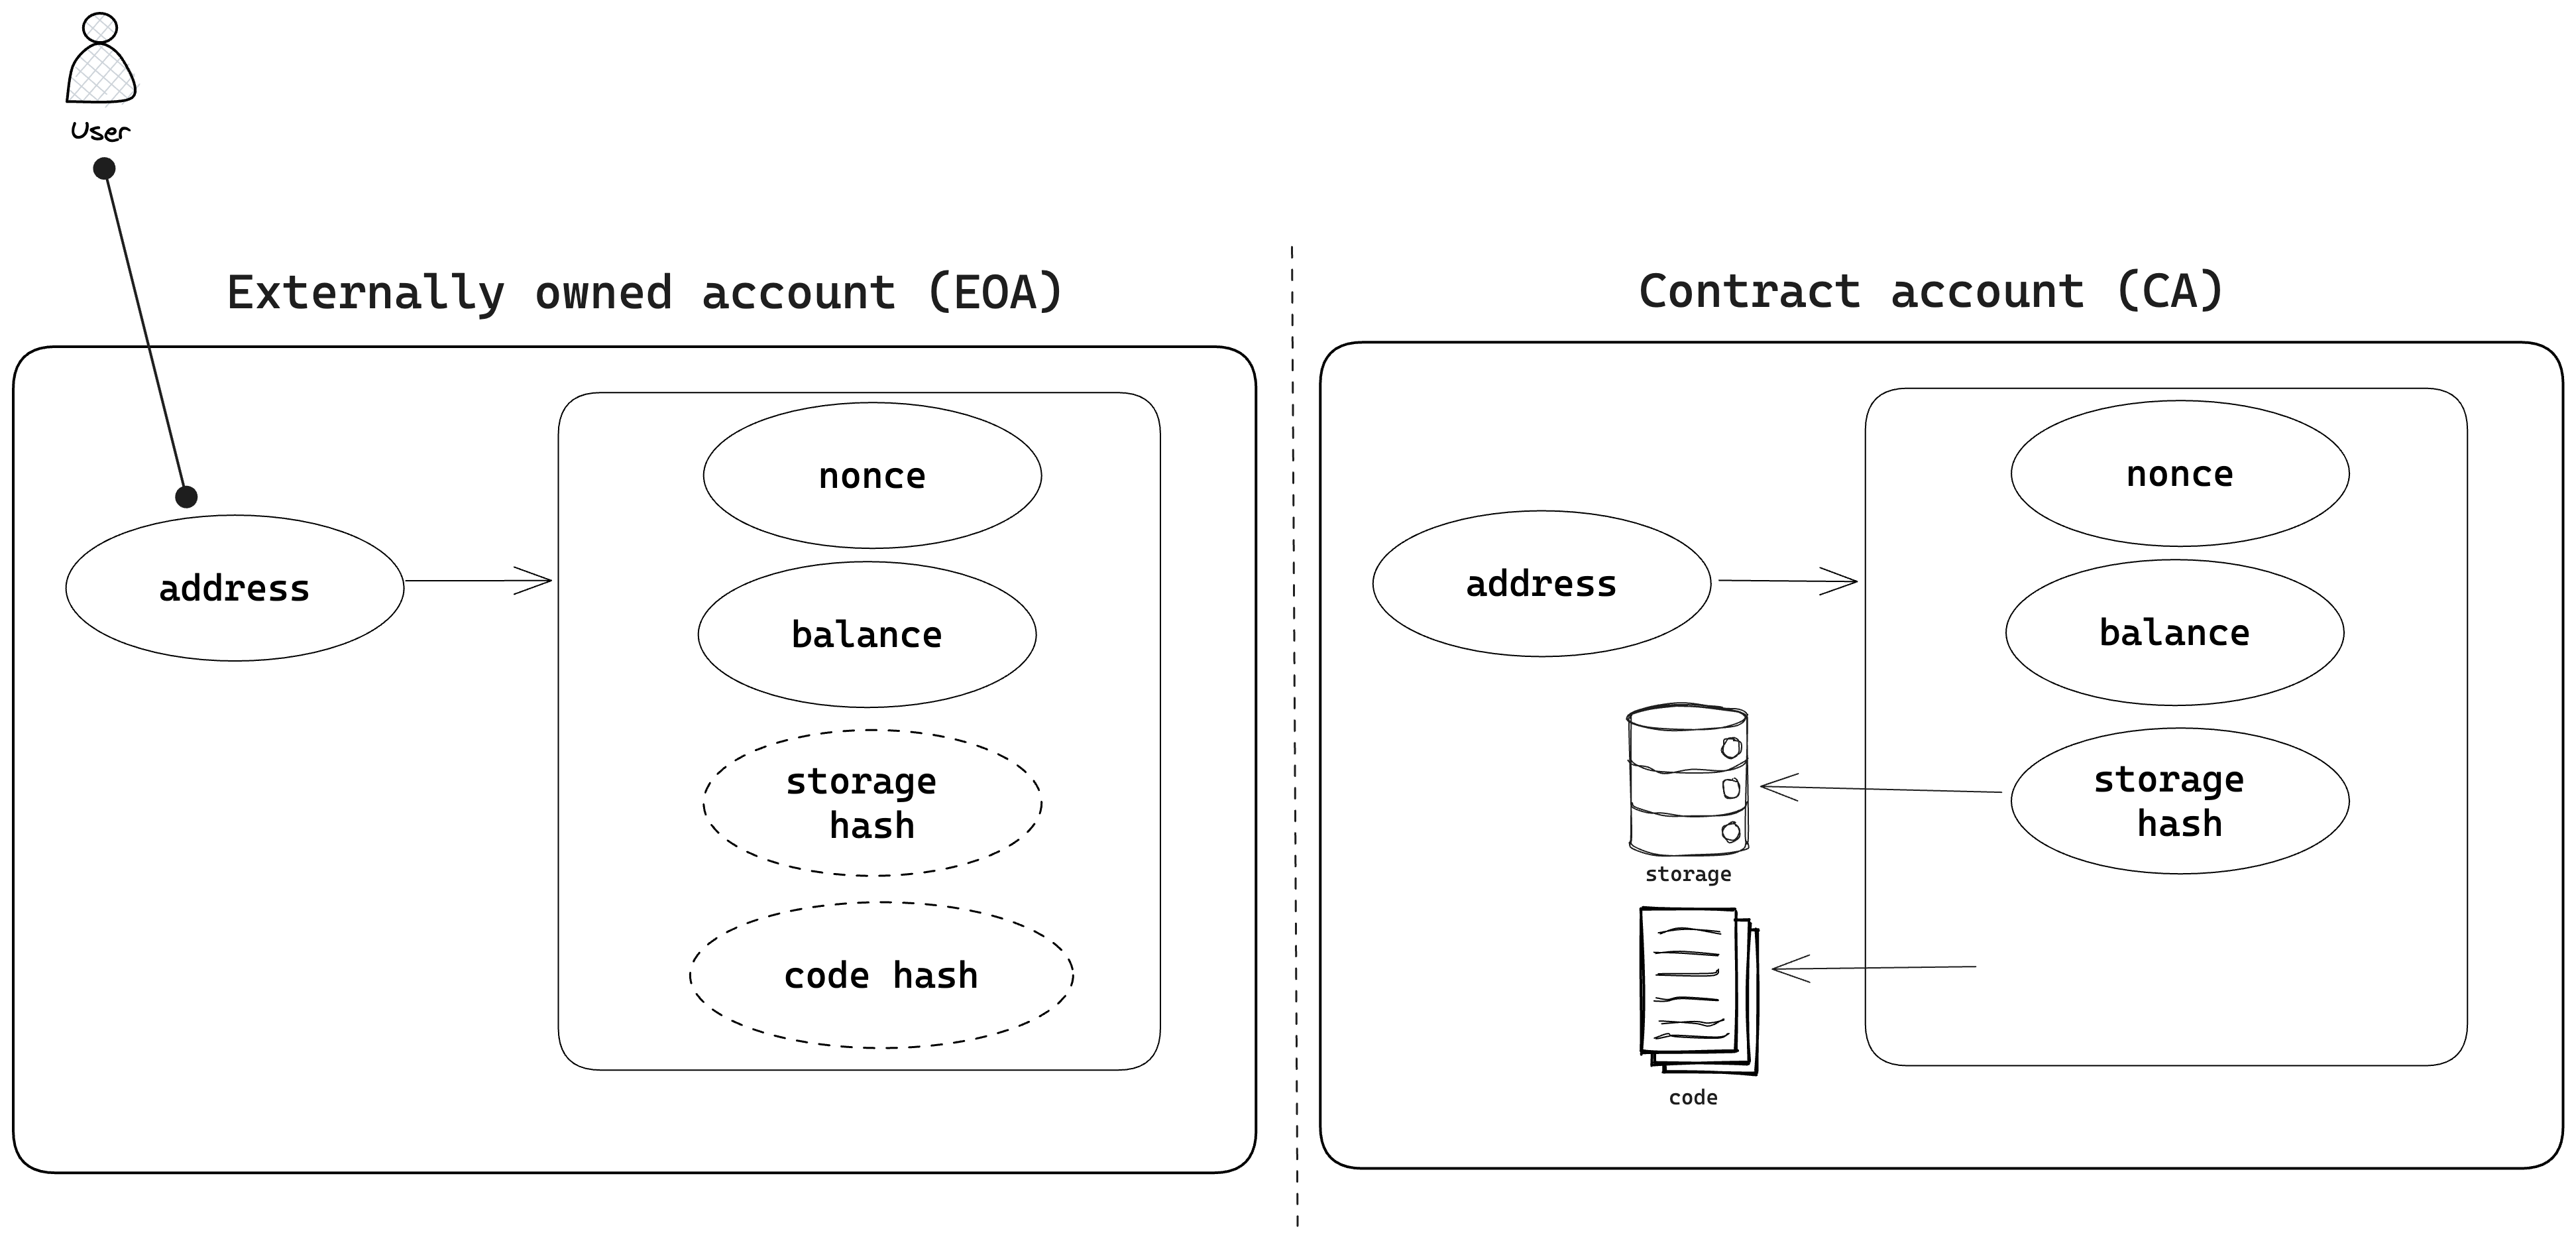
\includegraphics[width=.5\textwidth]{./images/account-types.png}
  \caption{Tipos de conta no Ethereum}
  \label{fig:fig1}
\end{figure}

Apenas as EOAs têm a capacidade de iniciar transações. Uma transação contém os seguintes campos:
\textit{nonce}, que também denota a quantidade de transações enviadas por essa conta, \textit{from}
- a EOA que assina a transação, \textit{recipient} - o endereço da conta de destino (se for uma
EOA, transferirá ETH, se for uma CA, acionará o contrato inteligente da CA), \textit{value} - a
quantidade de ETH a ser transferida para o destinatário em WEI, \textit{signature} - a assinatura
gerada com a chave privada da EOA que está transmitindo a transação\cite{15}. Existem ainda campos
adicionais relacionados ao gás\cite{6}, que não serão discutidos neste artigo.

As EOAs são controladas exclusivamente por chaves privadas que utilizam o esquema de assinatura
ECDSA\cite{17}. Essa restrição limita sua utilidade, pois para usá-las de forma segura, os usuários
precisam de conhecimento técnico para armazenar e utilizar chaves privadas. Além disso, a
usabilidade é restrita pela necessidade de assinar cada transação em tempo real, o que torna
impraticável a realização de pagamentos automáticos pré-autorizados. Outra consideração importante
é que o algoritmo ECDSA pode se tornar obsoleto com o avanço da computação quântica\cite{18}.

A AA é uma inovação proposta para o Ethereum com a finalidade de consolidar os dois tipos de contas
existentes: External Owned Accounts (EOAs) e Contract Accounts (CAs). O intuito primordial da AA é
oferecer aos usuários a alternativa de utilizar CAs, ao invés de EOAs, como suas contas primárias,
desvinculando, desta maneira, a ligação intrínseca das contas auto-custodiadas com o esquema de
assinatura ECDSA.

Essa transformação acarreta um aumento significativo na flexibilidade, possibilitando a criação de
contas com autenticação multi-assinaturas, autenticação de dois fatores, fixação de limites para
saques e habilitação de pagamentos automáticos\cite{26,9,12}. O impacto da inovação fornecida pela
AA é análogo à revolução que os Cartões Virtuais Revolut\cite{24} geraram no âmbito dos cartões de
crédito.

Foram propostas diversas abordagens para a implementação da AA no Ethereum\cite{25, 26}. A proposta
EIP-4337, no entanto, se destacou por prescindir de qualquer modificação na camada de protocolo do
Ethereum, razão pela qual nos referimos a ela como ERC daqui em diante. A ERC-4337 introduz uma
estrutura que descreve uma operação de usuário, designada como \textit{UserOperation}\cite{5}. É
importante salientar que, para evitar confusões terminológicas, este objeto não recebe a
denominação de transação, embora contenha, assim como uma transação, os campos previamente
mencionados, com algumas variações e acréscimos. Detalharemos essas questões na seção de
implementação técnica.

Os usuários submetem mensagens \textit{off-chain} que contêm o objeto \textit{UserOperation} para
um \textit{mempool} exclusivamente reservado para mensagens que incluem objetos
\textit{UserOperation}. Participantes conhecidos como \textit{bundlers} são incumbidos de ler as
mensagens recebidas pelo \textit{mempool}, coletá-las e agrupá-las em uma única transação.
Subsequentemente, realizam uma chamada para um método chamado \textit{handleOps} em um contrato
especial denominado \textit{EntryPoint}. Este contrato é responsável por executar essas transações
agrupadas e, consequentemente, inseri-las em um bloco na rede\cite{5}.

\begin{figure}[ht]
  \centering
  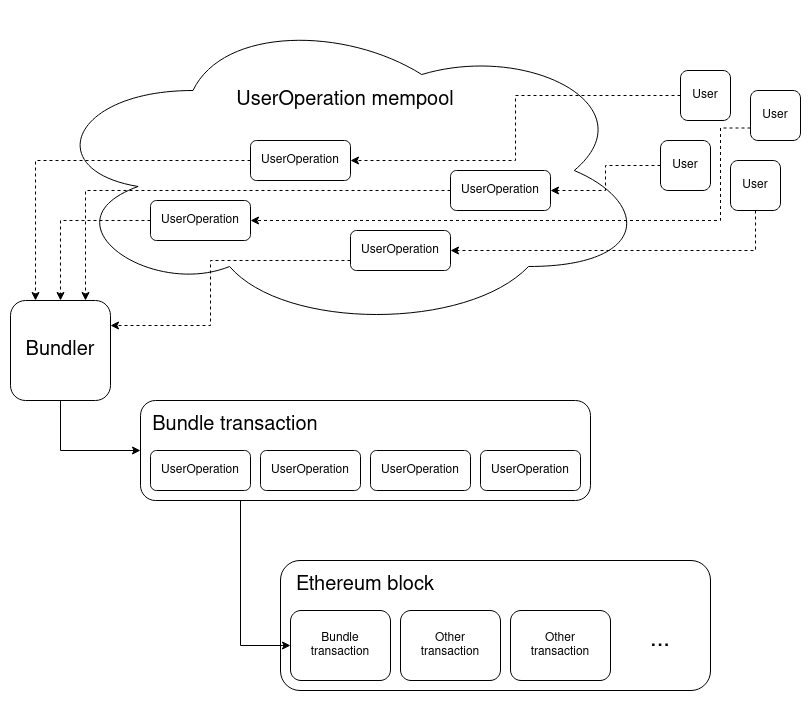
\includegraphics[width=.5\textwidth]{./images/user-operation-meenpool.png}
  \caption{UserOperation meempool}
  \label{fig:fig2}
\end{figure}

A chamada para o método \textit{handleOps} executará chamadas para os contratos inteligentes
associados às contas relacionadas aos objetos \textit{UserOperation}. O contrato inteligente de
cada conta é responsável por implementar a lógica de execução da transação e validar sua
legitimidade. Devido a EVM ser \textit{Turing-complete}, é possível criar lógicas de execução de
transações arbitrárias. Na próxima seção, proporemos uma implementação de contrato inteligente que
pode ser adotada por contas compatíveis com AA para habilitar pagamentos automatizados.

\bibliographystyle{sbc} \bibliography{tcc}
\end{document}

